\section{QUIC Adaptions}\label{sec:quic_adaptions}
As was already mentioned in the previous chapter, our setup requires some adaptations
to the quic-go library.
One initial change necessary was to turn off packet en- and decryption, 
that is happening within quic-go.
Given that we operate on the QUIC-header data within the eBPF program, we need access 
to fields that are encrypted using QUIC header-protection.
For obvious reasons sending unencrypted packets is not something that would be wanted in 
a production environment, but for our exemplary setup, it is unproblematic. 
An alternative would be to ``push down'' en- and decryption onto a smartNIC using a 
hardware offload, but at the time of writing, there was no such offload available for QUIC\@. 
Given that such a hardware offload is added in the future, the en- and decryption can be
turned on again, which makes this change more of a temporary solution to show the feasibility
of our approach.

\subsection{Function-Pointer Style Additions}
Another type of change that we needed to introduce into the quic-go library is caused by 
connection state management.
We essentially added support for communication with the eBPF program by using an 
approach similar to C-style function pointers.

On multiple locations, we added conditional function calls like the one depicted in 
\autoref{changes:function-pointer}.
The function that is called here will be defined by the developer of the relay and 
therefore allow for customizability without the need for changing the library itself.

\vspace{0.5cm}
\noindent\begin{minipage}{\textwidth}
\begin{lstlisting}[style=GoStyle, label=changes:function-pointer, caption=An example of a function-pointer addition to the quic-go library.]
    /* Function pointer call within actual quic-go code */
    if packet_setting.ConnectionUpdateBPFHandler != nil /* && potentially other conditions */ {
	    packet_setting.ConnectionUpdateBPFHandler(connId.Bytes(), uint8(connId.Len()), p.connection)
	}
\end{lstlisting}
\end{minipage}

\vspace{0.5cm}
\noindent\begin{minipage}{\textwidth}
\begin{lstlisting}[style=GoStyle, label=changes:signature-function-pointer, caption=Only the signature will be defined within the library itself.]
    /* Function pointer signature definition within additional config file */
	ConnectionUpdateBPFHandler      func(id []byte, l uint8, conn QuicConnection) = nil
\end{lstlisting}
\end{minipage}

The definition of the function that the developer of the relay wishes to be executed at specifically
defined points will be defined locally in the relay code and provided to the configuration of the quic-go library.
An example of how this could look like is shown in \autoref{changes:definition-function-pointer}.

\vspace{0.5cm}
\noindent\begin{minipage}{\textwidth}
\begin{lstlisting}[style=GoStyle, label=changes:definition-function-pointer, caption=An example of how the addition looks on the relay side.]
    /* Definition of the function within the local relay code */
    func localUpdateConnectionId(id []byte, l uint8, conn packet_setting.QuicConnection) {
        /* handle the connection update by interacting with the eBPF program */
    }   

    /* Providing the function to the quic-go library */
    func main() {
        /* ... */
        packet_setting.ConnectionUpdateBPFHandler = localUpdateConnectionId
        /* ... */
    }
\end{lstlisting}
\end{minipage}

The need for these additions arises since the eBPF program works with its own copy of the current state of a connection.
This, for example, includes the connection-id that will be used when changing the packet header before sending it out.
Since a connection-id can change, i.e.~be updated or retired, during the lifetime of a connection, we need a way to inform 
the eBPF program to no longer use outdated state-information.
These function-pointer style additions provide a minimal way of adding such functionality without limiting flexibility 
or adding too much application-specific code to the library itself, as would be the case if the library would access 
the eBPF-Maps directly.

% TODO: mention changes which are not function-pointer style
\subsection{Direct Changes to the Library}

\iffalse
% open stream with priority (+ datagram)

% turn off crypto (reaction to CRYPTO_TURNED_OFF flag)

% connection-id retirement specific stuff (switch to priority id)

% fixed sizes for fields e.g. conn id, stream-id, etc.(just for ease of development)

% e.g. only single stream frame inside packet (for ease of development) since general approach too complex for verifier?

% retransmission functions that open new stream with correct id

% registerBPFPacket function for connection

% prio enum. (prolly could be also given by relay dev) % TODO: not interessting enough i'd say
\fi

Besides the simple function-pointer style additions, we also had to make some direct changes to the library.
These include simplifications of the packet structure to make the implementation of a prototype easier 
but also changes that are necessary for the whole approach to work.
The necessary state changes mainly required internal state adjustments that would not be possible from outside 
the library because of missing access/visibility.
The optional turn-off for the packet en- and decryption based on the value of the \verb|CRYPTO_TURNED_OFF| flag
also required some direct changes to the library, but these will not be mentioned further since they are temporary
and not a focus of this chapter.

\subsubsection*{Simplifications of Packet Structure}
We added some changes to the quic-go library to make a prototype implementation easier.
The first one is that we fixed the sizes of some variable length fields like the connection-id or the stream-id.
This was mainly to avoid the need to figure out the correct sizes within the eBPF program as this would have 
resulted in approaches that would have to be very carefully turned into eBPF-compatible code due to verifier
restrictions.
Besides fixing the length of some fields, we also limit the number of frames per packet to one.
Normally a QUIC packet can contain multiple frames, especially stream-frames, but this would have required 
a packet traversal within the eBPF program that, again, would have been harder to implement considering all
verification constrictions.
Besides this additional complexity, for our usecase the ``singe-stream-frame-per-packet'' approach is not changing
a lot since the payload of one media packet will be split into multiple packets due to its size.
This means a single stream frame is likely already using up a whole packet, and multiple frames per packet would 
not be happening.

\subsubsection*{Stream Priorities}
Our approach relies on the fact that every packet has a priority value assigned to it.
In our case this priority value is stored within the connection-id.
Based on this, the first change, which is not only for simplification of our prototype implementation but is actually needed for 
our approach to work, is the addition of opening a stream with a specific priority.
Our assumptions define that the server is the one marking the packets with the correct priority, which in 
our case is realized by sending them over a specific stream.
Every stream is bound to a specific priority value, and our code changes will make sure that the connection-id
that is used for any packet sent on this stream will contain the correct priority value.
\autoref{fig:priority-stream} visualizes the setup as well as our rudimentary approach of saving the 
priority value as the first byte of the connection-id.

\vspace{0.5cm}
\begin{figure}[H]
    \centering
    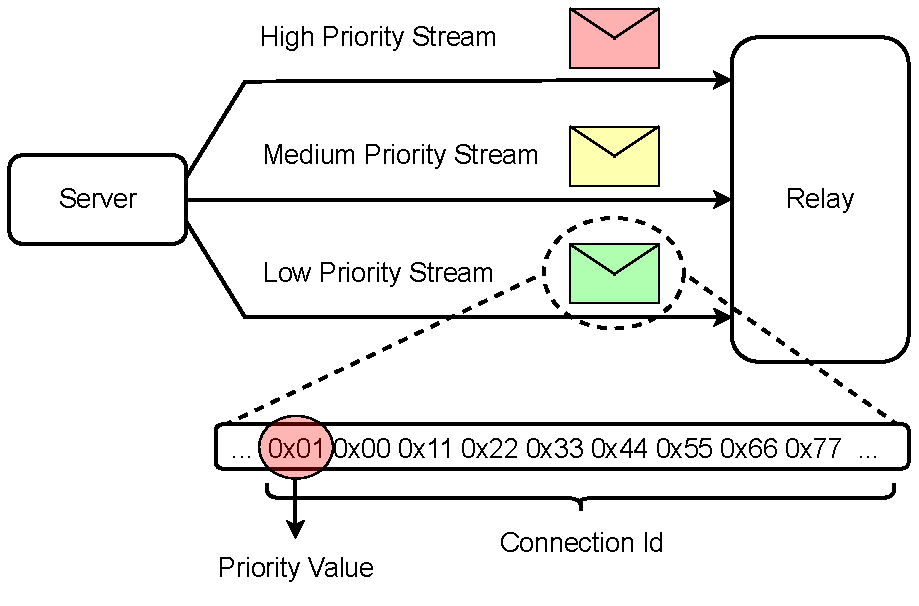
\includegraphics[width=0.7\textwidth]{figures/03_fast_relays/priority-streams.drawio.pdf}
    \caption[Streams with specific priorities]{The server opens streams with specific priorities, 
    which are then used to send packets with the corresponding priority.}\label{fig:priority-stream}
\end{figure}

This approach of having the priority value saved within the connection-id caused the need for another 
change in the library.
Due to the periodic change/retirement of connection-ids, we need to make sure that at any point in time, there 
exists one connection-id for each priority within the connection.
Otherwise, we might be unable to mark a packet with the correct priority.
This led us to introduce some additional logic to the code that is executing the retirement of connection-ids.
There, we will make sure that before a connection-id is retired, either one with the same priority value
already exists or is created.
This solves the problem of not being able to mark a packet with the correct priority.

\subsubsection*{Retransmission}
Another direct change that is needed is that of a specific \verb|OnLost| function for packets that 
have been forwarded by the eBPF program.
Since the relay state is not necessarily aligned with the server state, and the relay does not know
about the stream a packet was sent on, it is not possible to reuse the plain \verb|OnLost| function
of the quic-go library.
This is because the plain \verb|OnLost| function would lookup the stream corresponding to the provided stream-id and 
retransmit the packet on there, but the stream for the given id might not exist within the relay stream-pool.
Instead, our new function needs to look up the stream-id of the lost packet and open a new stream with
the same stream-id, ensuring that the client correctly receives the retransmission.
Besides the stream-id, the created stream-object should also have the same remaining stream-state
as the original stream (e.g.~offset-information).  
When a retransmission happens, the relay also needs to tell the underlying eBPF program that a packet is part of a 
retransmission and that, even if a stream was actually created by the relay, the egress program should treat it like 
it was created by the server.
That last part is necessary for the stream-id translation part of the egress program, which is explained further
in~\autoref{sec:client-egress}, to work correctly.
This functionality of informing the eBPF program about the retransmission, however, is again realized by a 
function-pointer style addition and thus designed by the relay developer.

\subsubsection*{Visible Endpoint for Packet Registration}
The last direct change that we added was the introduction of an additional function \verb|RegisterBPFPacket| 
on a quic-go connection object that allows the relay to register a packet.
Since the packet registration requires access to internal state of the connection, this also needed to be 
done as an actual change to the library.
Now the relay can just read the necessary information of a packet that needs to be registered
from the eBPF-maps and then pass it on to this function which will handle the registration.
This also provides a good separation between the Go code that handles eBPF communication and the actual
QUIC connection handling.